\section{Análisis de Centralidad}

\begin{figure}[H]
    \centerfloat
    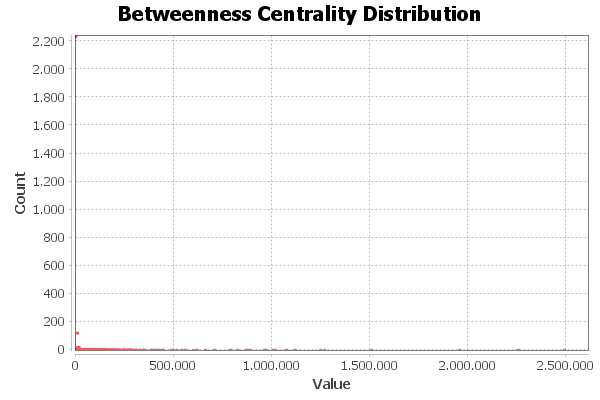
\includegraphics[width=0.9\textwidth]{img/resultados/distanciaGrafo/Betweenness Centrality Distribution.png}
    \caption{Distribución de valores de intermediación.}
\end{figure}

\begin{figure}[H]
    \centering
    \resizebox{0.9\columnwidth}{!}{%
    \begin{tabular}{| l | l | l | l |} 
        \hline
        \textbf{Centralidad de Grado} & \textbf{Intermediación} & \textbf{Cercanía} & \textbf{Vector propio} \\
        \Xhline{2\arrayrulewidth}
        \textbf{7237} - 216 & 	\textbf{7199} - 2,612,617 & \textbf{7199} - 0.2907 & 	\textbf{7237} - 1.0000  \\
        \hline
        \textbf{3530} - 175 & 	\textbf{7237} - 2,486,453 & 	\textbf{7237} - 0.2856 & \textbf{3240} - 0.7149  \\
        \hline
        \textbf{4785} - 174 & 	\textbf{2854} - 2,253,302 & 	\textbf{4356} - 0.2816 & 	\textbf{3597} - 0.7052  \\
        \hline
        \textbf{524}   - 172 & 	\textbf{4356} - 1,953,690 & 	\textbf{2854} - 0.2803 & 	\textbf{763}   - 0.6555  \\
        \hline
        \textbf{3450} - 159 & \textbf{6101} - 1,504,994 & 	\textbf{5454} - 0.2798 & 	\textbf{2083} - 0.5940  \\
        \hline
    \end{tabular}
    }
    \caption{Tabla de actores más relevantes (identificador-valor).}
\end{figure}